\clearpage
\section{附加实验，形态学补全与原方案比较}
\subsection{补全方法与比较条件}

原方案填孔后，00570 的嘴部仍有向外连通的缺口。这类缺失属于外部背景的一部分，普通填孔会保留它。新增方法先保留最大连通域，再进行膨胀、填孔和腐蚀，尝试用膨胀封住较窄的开口，填充内部区域后再收回扩张的外缘。

本节将前文的最大连通域与填孔记为原方法，将新增流程记为补全方法。两者共用训练颜色统计、$k=1.25$ 和原始图像尺寸，正类与忽略区域的定义也保持一致。补全使用 $41\times41$ 椭圆核，膨胀和腐蚀各执行一次。处理前在图像外围补零，全部步骤结束后再裁回原尺寸，避免图像边缘影响贴边目标的腐蚀结果。

核大小来自验证集上的 15 组候选，包含纯阈值、原方法、原有闭运算参考，以及两种新增补全流程各自的 6 个核大小，取值为 5、9、15、21、31、41。选择规则是在原方法全局 F1 的基础上最多下降 0.01，再在符合条件的候选中选择 Recall 最高的一组。这里优先考虑减少缺口，与前文按最高 F1 选参的目标有所区别。

\begin{table}[H]
\centering\small
\caption{原方法与补全方法的验证结果，单位为百分比}\label{tab:morphvalidation}
\begin{tabular}{lrrrr}
\toprule
方法 & Precision & Recall & F1 & IoU \\
\midrule
原方法 & 64.86 & 82.70 & 72.70 & 57.11 \\
补全方法 & 61.77 & 86.22 & 71.98 & 56.22 \\
变化，百分点 & -3.09 & +3.52 & -0.72 & -0.89 \\
\bottomrule
\end{tabular}
\end{table}

验证集上，补全方法减少 78,523 个漏检像素，并增加 190,636 个误检像素。它满足允许的 F1 损失范围，体现的是覆盖率与误检之间的取舍。

本次测量固定新增配置后，先重新生成两种方法的验证预测，再评价原来的 32 张测试图。验证计数与发布记录完全一致，同源码中的原方法也与原实验的 64 张验证和测试预测逐像素一致。原图、真值、忽略区域、指标公式和边界带宽均沿用前文设置。

新增方法的设计已经参考过测试图 00570 的反馈，因此本节作为开发后的附加对比。前文保留原方案的独立测试结果，本节使用已有测试图观察补全效果，另留图像才可以再次检验新方法的泛化表现。

\subsection{总体结果与新增区域}

\begin{table}[H]
\centering\small
\caption{原测试集上两种固定方法的附加对比，指标单位为百分比}\label{tab:morphtest}
\begin{tabular}{lrrr}
\toprule
指标 & 原方法 & 补全方法 & 变化，百分点 \\
\midrule
Accuracy & 83.940 & 83.098 & -0.842 \\
Precision & 66.425 & 63.628 & -2.797 \\
Recall & 75.548 & 79.549 & +4.001 \\
F1 & 70.693 & 70.703 & +0.010 \\
IoU & 54.671 & 54.683 & +0.012 \\
\bottomrule
\end{tabular}
\end{table}

\begin{table}[H]
\centering\small
\caption{附加对比的混淆计数}\label{tab:morphcounts}
\begin{tabular}{lrrrr}
\toprule
方法 & TP & FP & TN & FN \\
\midrule
原方法 & 1,624,818 & 821,271 & 5,416,615 & 525,904 \\
补全方法 & 1,710,868 & 977,980 & 5,259,906 & 439,854 \\
\bottomrule
\end{tabular}
\end{table}

补全后 Recall 提高了 4.00 个百分点，原有漏检减少 16.36\%。与此同时，FP 增加了 19.08\%，Precision 下降 2.80 个百分点。总体 F1 和 IoU 几乎保持原值，所以这次更新主要改变了覆盖范围。

将两张预测掩膜直接作差，这批图像中原来选出的像素全部保留，共新增 242,759 个前景像素，其中 86,050 个属于脸部，156,709 个属于非脸部，新增区域中正确部分占 35.45\%。这一结果解释了为什么脸部覆盖更完整，整体 F1 却只有很小变化。

\begin{table}[H]
\centering\small
\caption{补全新增像素的语义来源}\label{tab:morphsemantic}
\begin{tabular}{lrr}
\toprule
真实区域 & 新增正确脸部像素 & 新增误检像素 \\
\midrule
皮肤与鼻子 & 68,758 & 0 \\
眼、眉、口腔与嘴唇 & 17,292 & 0 \\
头发 & 0 & 116,896 \\
背景 & 0 & 20,534 \\
脖颈 & 0 & 13,043 \\
其他负类 & 0 & 6,236 \\
\bottomrule
\end{tabular}
\end{table}

五官组的召回率从 68.32\% 提高到 79.11\%，说明更强的补全确实恢复了部分原来遗漏的内部结构。新增误检则以头发为主，占新增 FP 的 74.59\%。形态学根据区域连通和核大小决定补入哪里，当头发与主体相连时，也会沿着这些错误候选继续补全。

\clearpage
\subsection{补全收益与误检扩大的图像对照}

以下保留反馈样例 00570，并从全部逐图结果中选择漏检减少最多的 00537、误检增加最多的 00578 和 F1 下降最多的 00647。每张对照图展示同一原图、人工真值、新旧预测和对应误差，绿色为正确检出，红色为误检，蓝色为漏检。

00570 的嘴部横向缺口减少，新增 4,367 个正确像素和 1,247 个误检像素，F1 从 0.759 提高到 0.803，如图~\ref{fig:morph570} 所示。额头和眼周仍有较大的漏检区域，说明当前核能够修补部分开口，而较大的缺失还受到原始候选形状的限制。

\begin{figure}[H]
\centering
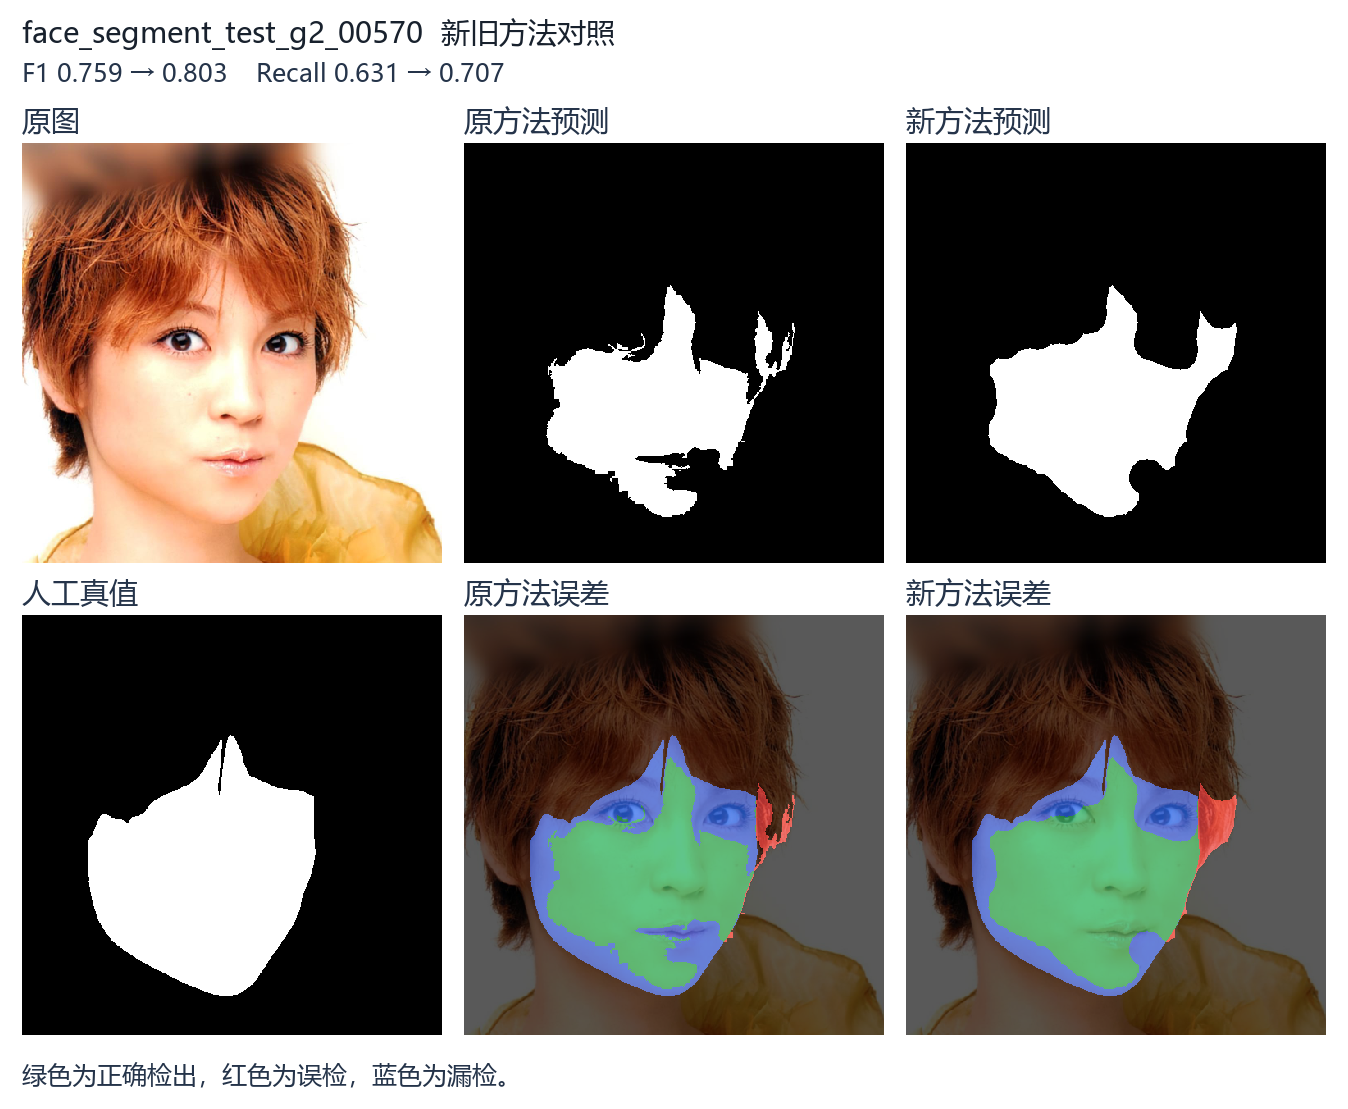
\includegraphics[width=0.94\textwidth]{morphology_00570.png}
\caption{00570 的嘴部缺口减少，额头与眼周仍有漏检}
\label{fig:morph570}
\end{figure}

\clearpage
00537 的补全收益最明显，如图~\ref{fig:morph537} 所示。原来脸部右侧的大块缺失被补回，漏检减少 25,174 个像素，Recall 从 52.98\% 提高到 99.89\%，F1 从 0.584 提高到 0.803。该图也增加了 11,119 个误检像素，主要可见于脸侧头发和下部区域。正确主体已经位于较连贯的外轮廓内时，补全可以恢复较大面积的脸部。

\begin{figure}[H]
\centering
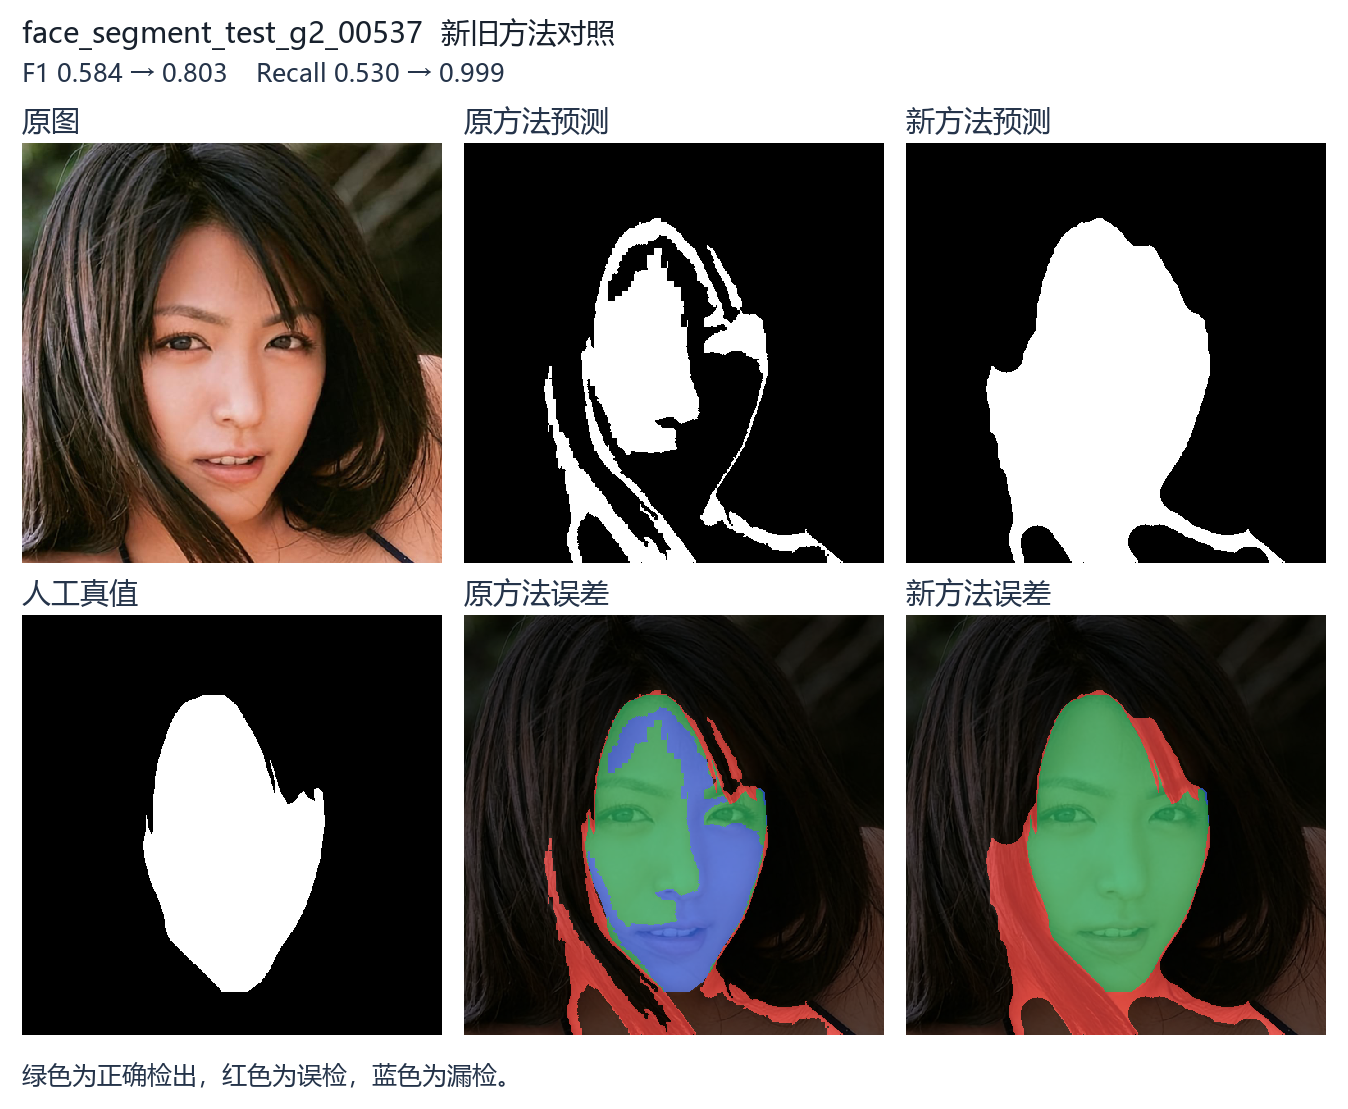
\includegraphics[width=0.94\textwidth]{morphology_00537.png}
\caption{00537 找回最多的脸部像素，同时扩大了脸侧误检}
\label{fig:morph537}
\end{figure}

\clearpage
00578 的误检增加最多，如图~\ref{fig:morph578} 所示。原方法已将头发选为主体，新方法沿着这块区域继续补全，新增 22,692 个误检像素，只恢复 1,505 个正确像素。F1 从 0.103 变为 0.105，脸部主体仍然大面积缺失。结果在外观上更加连续，主要覆盖的却仍是头发。

\begin{figure}[H]
\centering
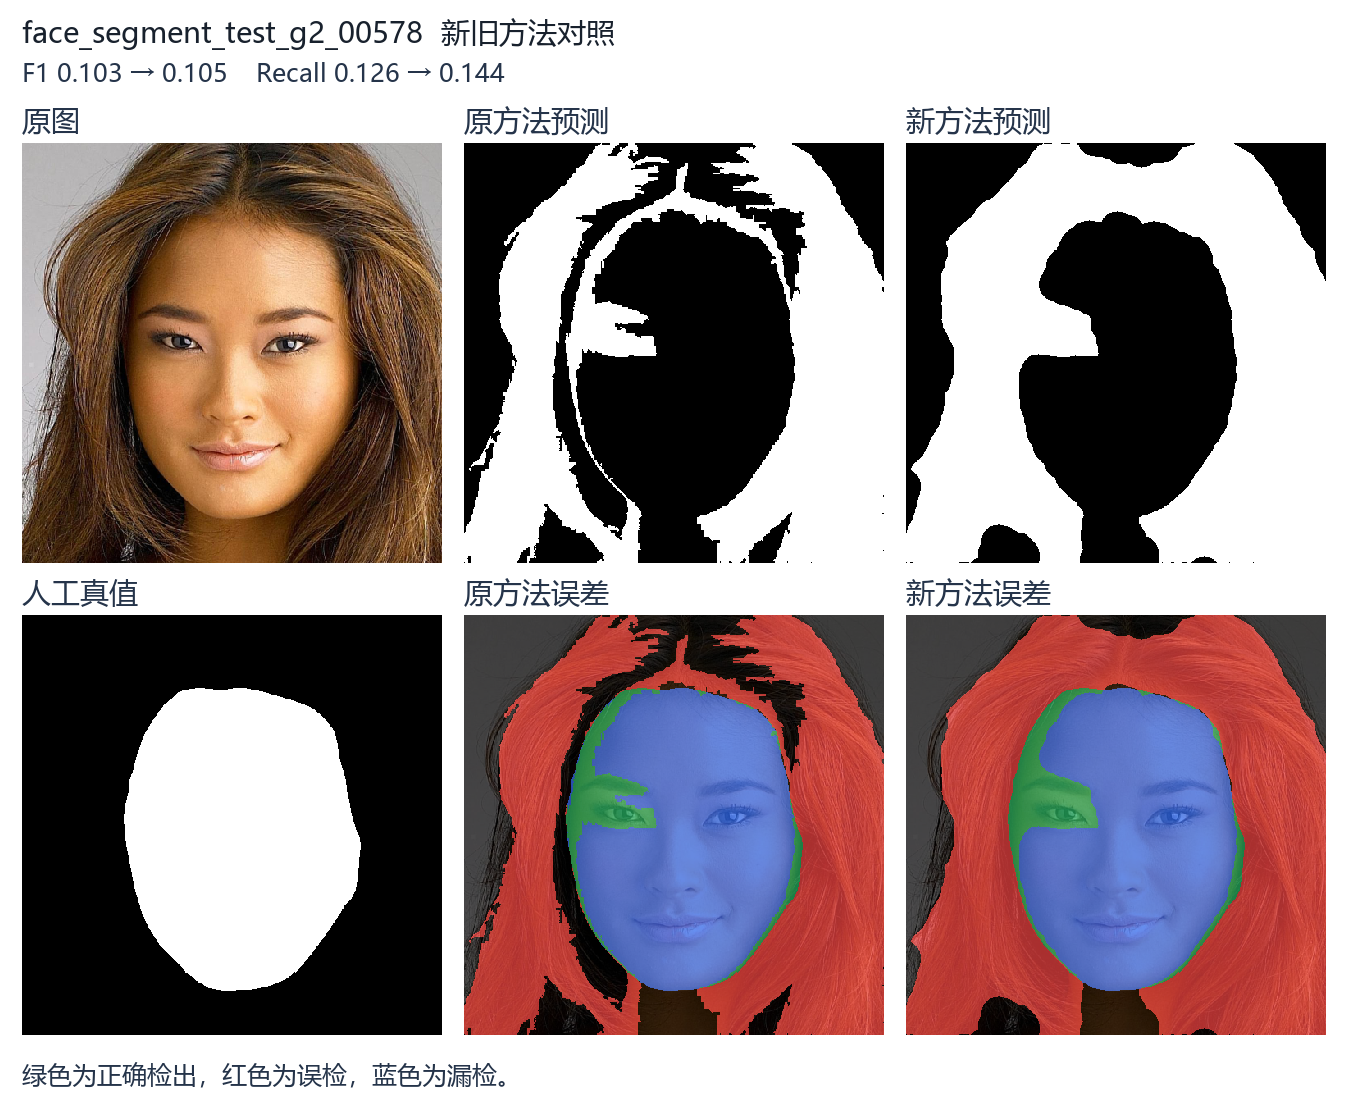
\includegraphics[width=0.94\textwidth]{morphology_00578.png}
\caption{00578 中头发误检扩大，脸部主体仍然缺失}
\label{fig:morph578}
\end{figure}

\clearpage
00647 则表现为原有覆盖已经较充分，继续补全主要增加了周围错误区域，如图~\ref{fig:morph647} 所示。原方法的 Recall 已达到 99.58\%，新方法只多恢复 117 个正确像素，却增加 19,907 个误检像素，F1 从 0.720 降到 0.662。对于本来就接近完整的脸部，统一使用大核会付出更多误检代价。

\begin{figure}[H]
\centering
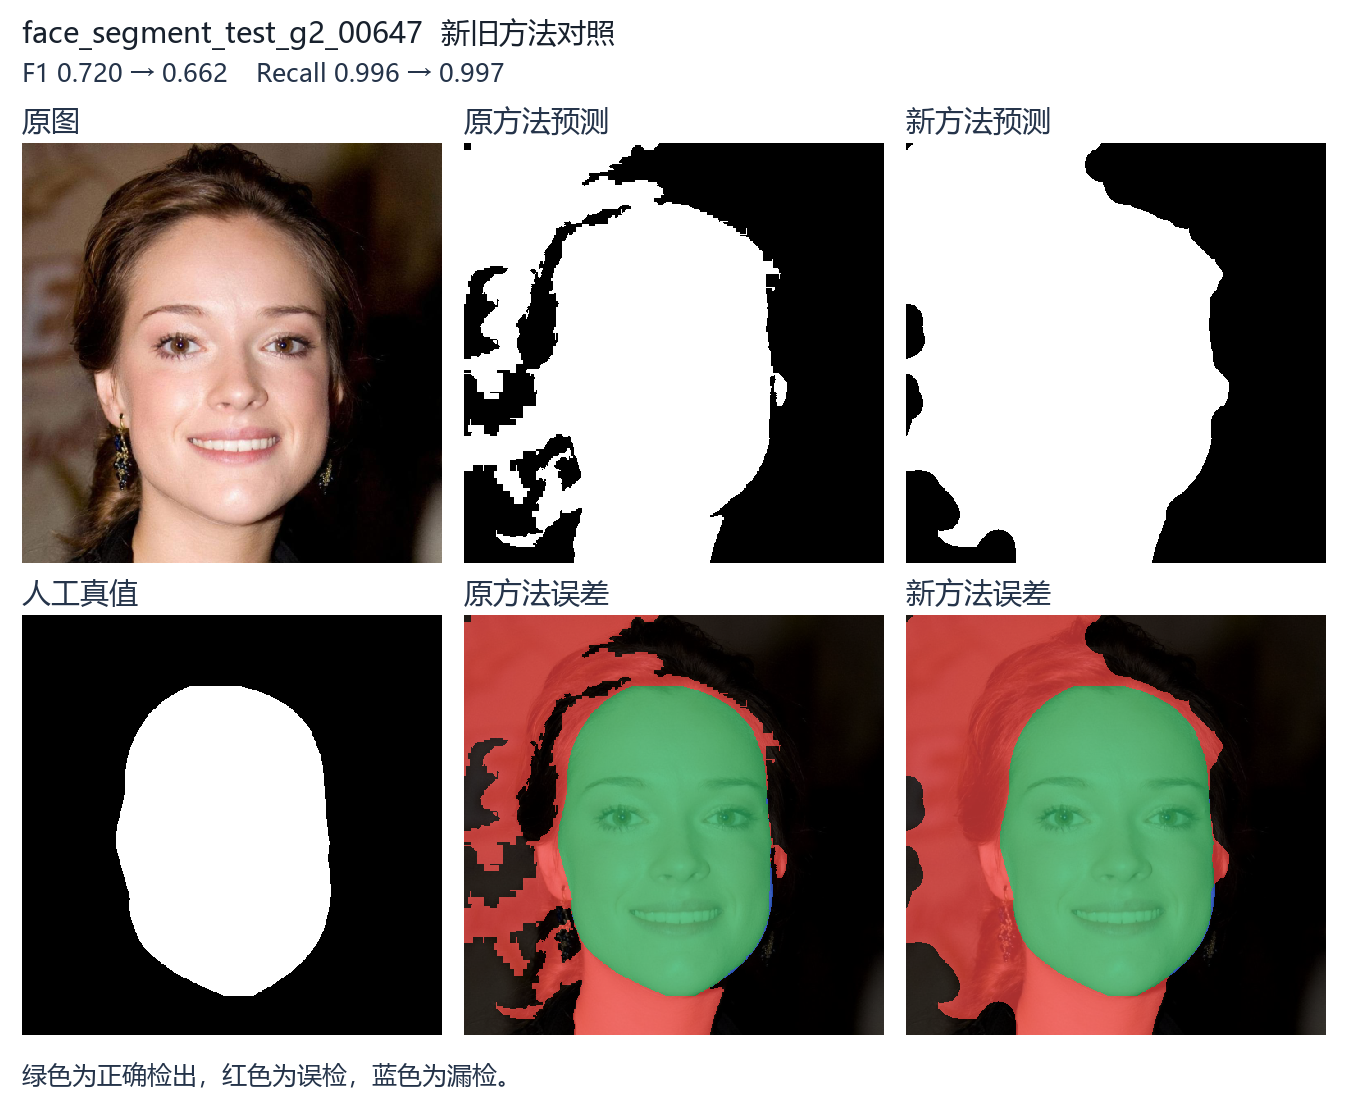
\includegraphics[width=0.94\textwidth]{morphology_00647.png}
\caption{00647 的脸部已基本检出，补全主要扩大了非脸部区域}
\label{fig:morph647}
\end{figure}

\clearpage
\subsection{逐图变化、边界与后续改进}

32 张图中有 19 张 F1 提高，13 张下降，逐图平均 F1 从 0.681 提高到 0.690。图~\ref{fig:morphpaired} 将每张图作为一个点，左侧直接比较 F1，右侧观察 Recall 与 Precision 如何共同变化。00537 的提升较大，00647 则体现了覆盖已经充分时继续扩张的代价，整体均值因此只能概括其中一部分情况。

\begin{figure}[H]
\centering
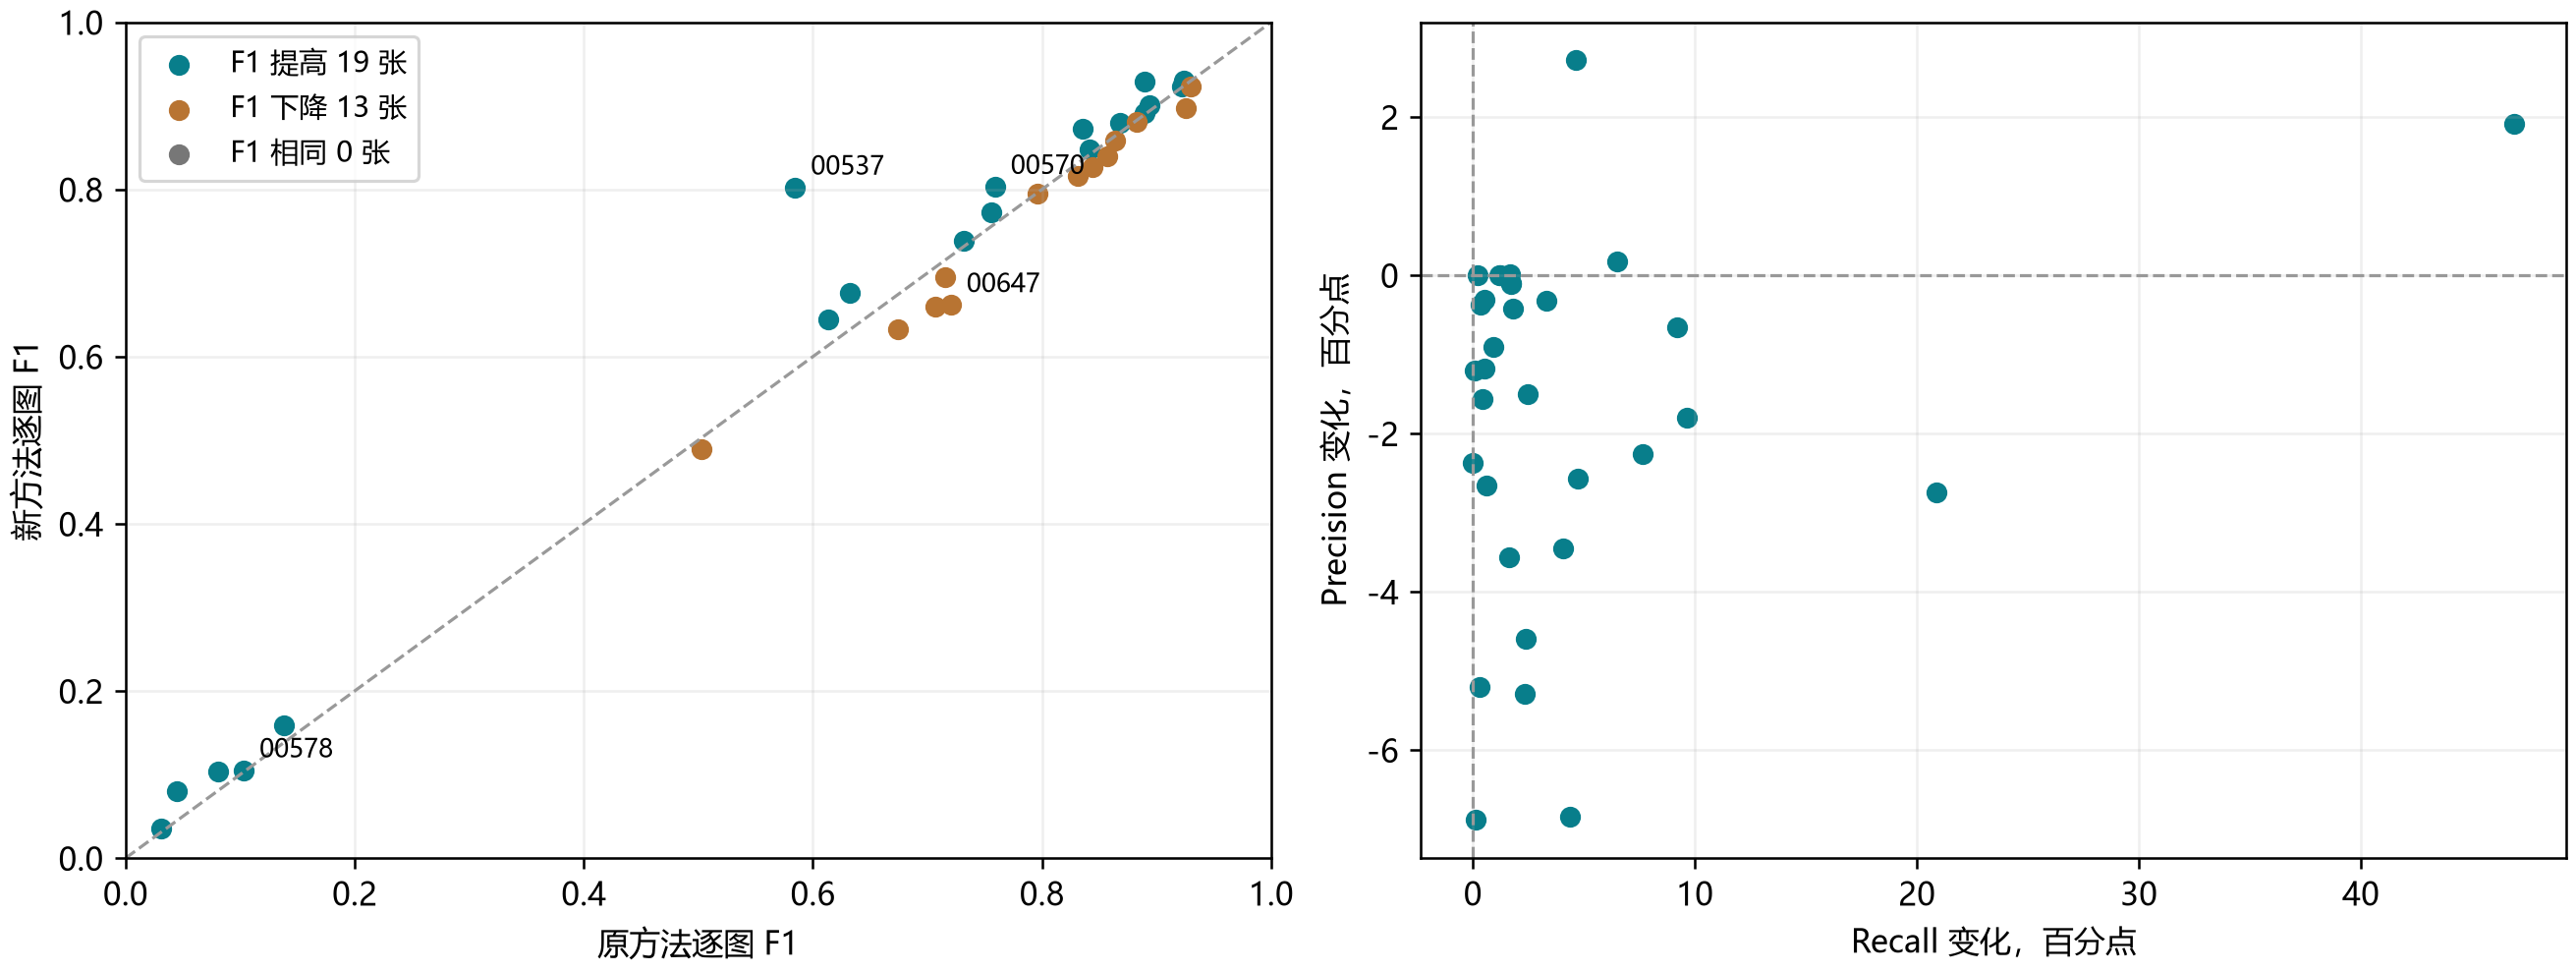
\includegraphics[width=\textwidth]{morphology_paired_changes.png}
\caption{逐图 F1 对照，以及覆盖率变化与预测准确程度变化的关系}
\label{fig:morphpaired}
\end{figure}

沿用 14 像素内侧边界带，逐图 Boundary IoU 平均由 0.2328 降到 0.2267。补全使部分缺口收拢，同时也改变了脸部外侧的轮廓。结合头发误检的增长，可以看到区域更连续与边界更贴合需要分别检查。

按图像配对重采样 10,000 次，种子仍为 42，总体 F1 差值的 95\% 区间为 -1.27 至 +1.66 个百分点，逐图平均 F1 差值的区间为 -0.45 至 +2.66 个百分点。这些区间描述当前样本组成变化时的波动，与观察到的总体 F1 基本持平一致。

补全也没有解决所有候选不足的问题。原来的失败图 00609 的 Recall 仅由 1.59\% 变为 1.78\%，00718 则由 5.12\% 变为 9.78\%，仍存在大面积漏检。颜色候选本身覆盖很少或区域选择已经偏离脸部时，扩大形态学核的作用有限。

后续可以先在验证集比较按候选形状和开口大小控制的局部补全，并同时记录恢复的脸部像素和新增的头发误检。对于已经完整的候选，应减少额外扩张，对于严重偏离脸部的候选，则应先改进颜色与区域判别。当前结果支持将补全作为减少缺口的一种取舍，若以总体 F1 为主要目标，原方法仍然是性能相近且边界均值略高的参考方案。
